% !TEX root = ../../Article.tex
\section{Android Application}

\subsection{3rd party libraries}
Gemalto provides a java library, IDGo800, for communicating and utilizing built-in methods with their smart cards.

\begin{aquote}{Gemalto.com \cite{GemaltoIDGo800}}
``IDGo 800 for Mobiles is a cryptographic middleware that supports the Gemalto IDPrime cards and Secure Elements on Mobile platforms: Contact and contactless smart cards, MicroSD cards, UICC-SIM cards, embedded Secure Elements (eSE) and Trusted Execution Environment (TEE).''
\end{aquote}

The part of IDGo800 SDK we are interested in is very small and enables us to send custom APDUs to micro SD smart cards.

We will be using the ``android.nfc'' package in order to communicate with NFC smart cards. This package is included in the standard Android SDK which in turns means that all Android devices with a NFC reader and minimum API level 9 \cite{androidNFCminSDK} can use our library.

\subsection{Application}
\label{sec:androidApp}

In section \ref{sec:designAndroidGoals} we described the goals of the framework. The first goal we will describe the implementation of is ``extendable'' or in other words, being able to send custom APDUs. Explaining how this is implemented will give a better understanding of how the framework is built up and makes it easier to understand the pre-implemented methods.

We used the same approach on the Android application as on the smart card application; an autonomous and easy to extend platform for tests. This resulted in a new library, ``smartcardlibrary'',  which sole purpose is to transmit APDUs as easily as possible along with some basic functionality.

\paragraph{Custom APDUs}\mbox{}\\
To send custom APDUs to a smart card,\texttt{CommunicationController} must be instantiated and the application must know the application identifier of the smart card application. Further the current activity must implement\\ \texttt{NfCSmartcardControllerInterface} or \texttt{MSDSmartcardControllerInterface} (depending on smart card type) in order to be notified when the transaction is complete. Before continuing one will need to call the methods \texttt{setupNFCController} or \texttt{setupmSDController} depending on the smart card. Listing \ref{lst:NFCLibraryExample} shows an example implementation on how an activity may utilize the library for sending custom commands to a NFC smart card.

\begin{lstlisting}[caption=Java code example showing how to send and receive commands to a NFC smart card., label=lst:NFCLibraryExample,escapechar=å]

public class PayloadActivity extends AppCompatActivity
    implements NFCSmartcardControllerInterface {
    CommunicationController cc = new CommunicationController();
    ...

    private void initNFCCommunication(){


        String AID = "0102030405060708090007";
        String hexMessage = "95404F3FB1";
        String INS = "06";
        String p1 = "00";
        String p2 = "00";
        cc.setupNFCController(this, this);
        cc.initNFCCommunication(AID, INS, p1, p2, hexMessage);
    }

    å@Overrideå
    public void nfcCallback(final String completionStatus){
        if(!completionStatus.equals("OK")){
            return;
        }
        StorageHandler stHandler =
            new StorageHandler(getApplicationContext());
        String response =
            stHandler.readFromFileAppDir(
                FilePaths.tempStorageFileName
            );
    }
}

\end{lstlisting}

In order for the library to perform an asynchronous transaction the library will temporary save the responses from the cards to a file only accessible by the running application. To retrieve the data the current activity should use the included \texttt{StorageHandler} class as used in listing \ref{lst:NFCLibraryExample}. The library also provides the class, \texttt{Converter}, for converting between Strings, hex and byte arrays.

\paragraph{Pre-implemented methods}\mbox{}\\
Recall the areas we want to cover from the beginning of the chapter. The functionality we have implemented so far are:

\begin{itemize}
    \item Bind smart card to mobile device.
    \item Encrypt/decrypt data using RSA key on card.
    \item Encrypt/decrypt data using AES key on card.
    \item Get public key of the smart card.
    \item Sign data using the public key of the smart card.
\end{itemize}

To use these functionalities one would only need to create an Android \texttt{Activity}, invoke either \texttt{\allowbreak setupNFCController(...)} or \texttt{setupmSDController(...)} (depending on smart card), and utilize the desired methods. In figure \ref{fig:instantiateflow} we can see how \texttt{CommunicationController} is designed to be the abstraction layer between Android activities and smart cards.


\begin{figure}[h!]
  \caption{Abstraction layer between Android activities and smart cards.}
  \label{fig:instantiateflow}
  \centering
    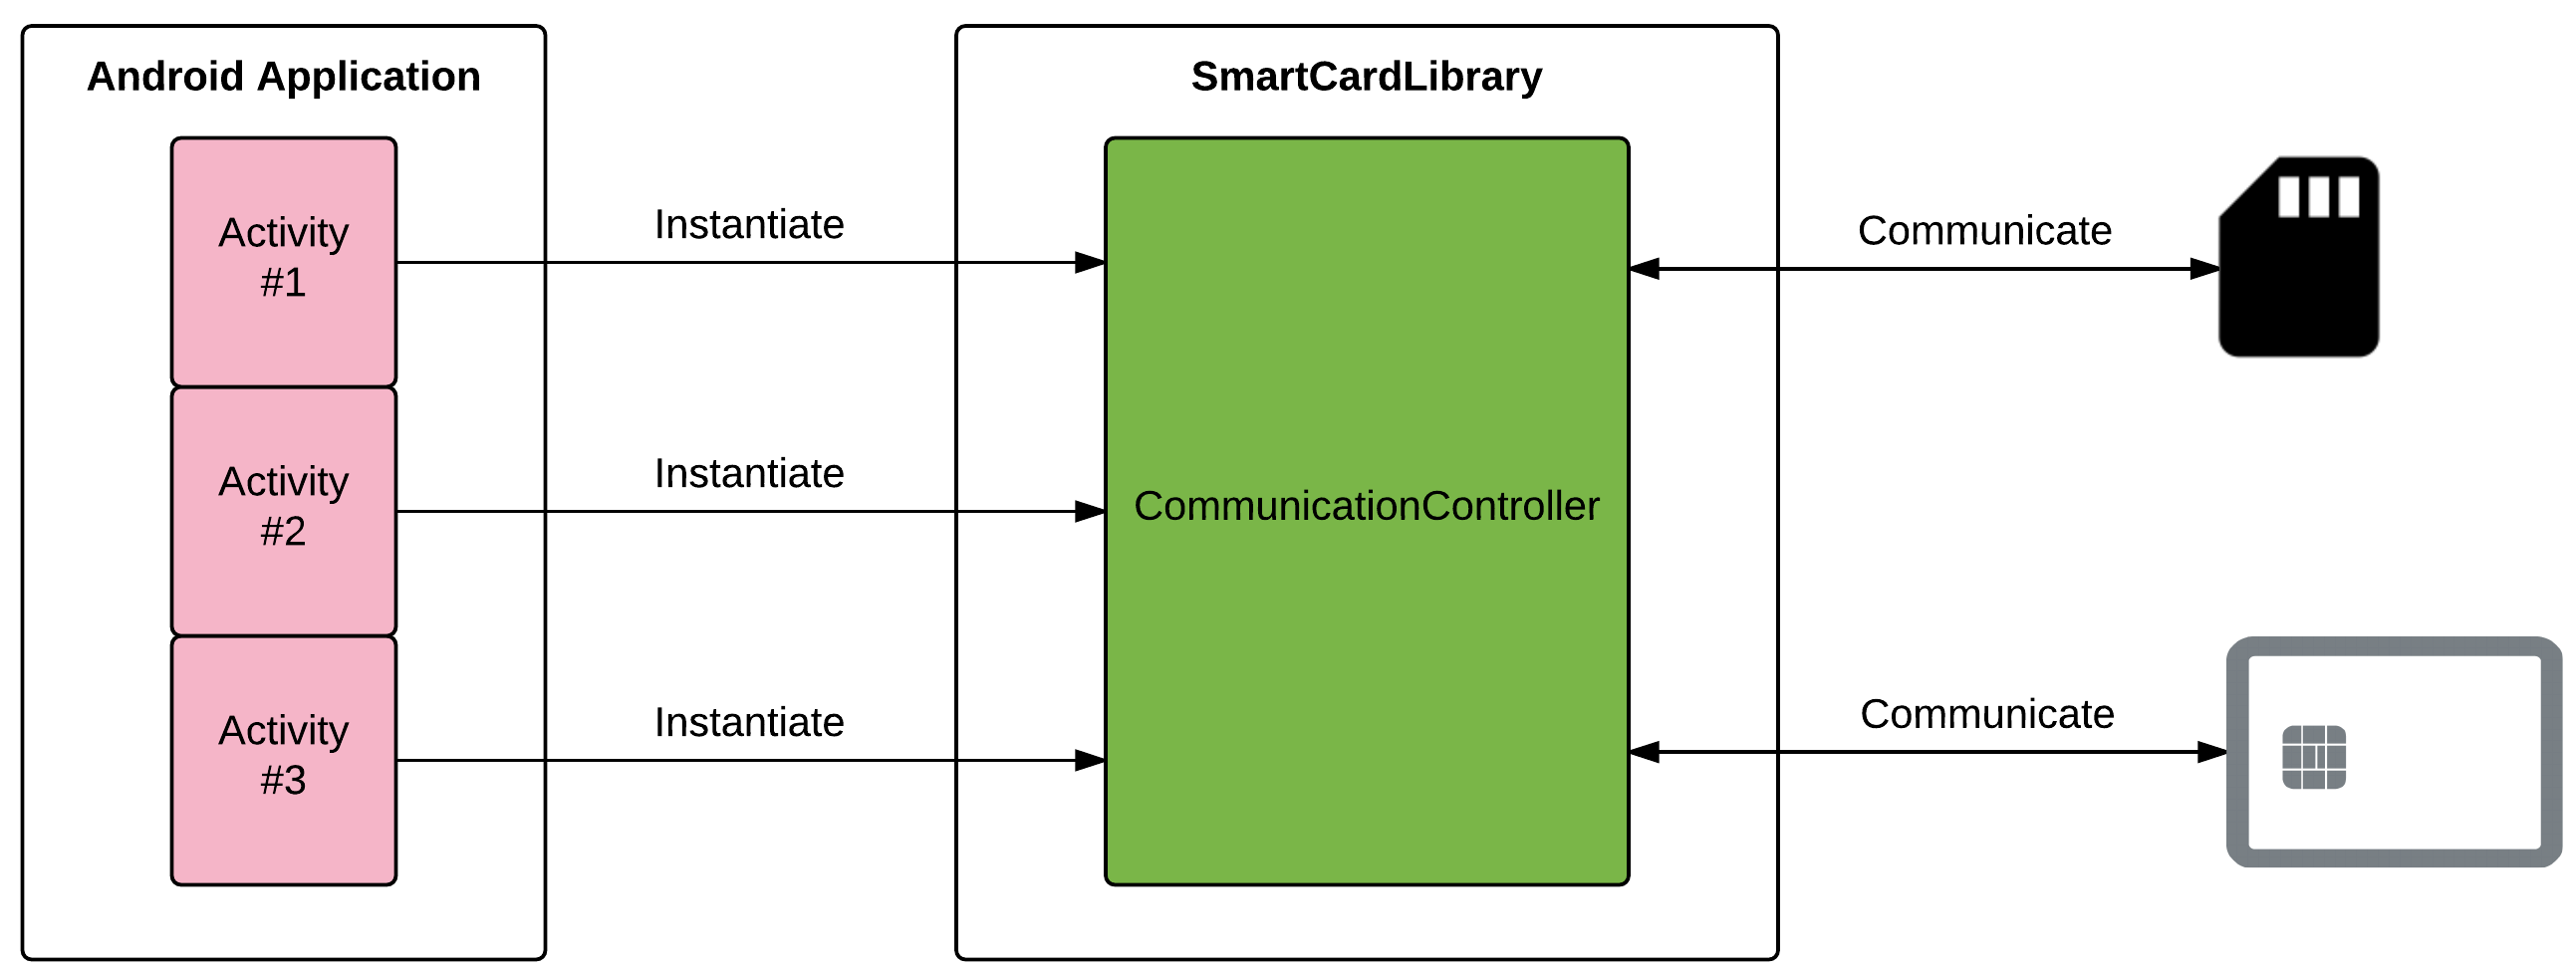
\includegraphics[width=0.95\textwidth]{images/Instantiate_flow.png}
\end{figure}

The methods available are:

\begin{itemize}
    \item public void disableNFC(...)
    \item public void signData(...)
    \item public void cryptoRSA(...)
    \item public void cryptoAES(...)
    \item public void getCardPubMod(...)
    \item public void getCardPubExp(...)
    \item public void bindingStepOne(...)
    \item public void bindingStepTwo(...)
    \item public void bindingStepThree(...)
\end{itemize}

The methods and their functionality should be self-explanatory except for the binding process. The binding process is designed in three steps. First step is to ask the smart card if it requires a PIN-code and how many attempts are left. Second step requires a PIN-code and if this is correct the smart card application will move on to step three. The last step is sending the public key of the mobile device and getting the verification package from section \ref{sec:proposedSolution}. More discussion on this matter in section \ref{sec:bindingcardandphone}.

Listing \ref{lst:NFCSigning} shows how an activity can use the \texttt{CommunicationController} to sign a simple message. The \texttt{signData(...)} method takes 3 parameters: CommunicationType, AID and the hex message to be signed. In the method \texttt{nfcCallback(...)} the developer are free to do whatever they want. Typically it is a good idea to check what the completeionStatus string is before trying to fetch the response data. Read appendix \ref{app:b} for all method signatures.

\begin{lstlisting}[caption=Java code example showing how to send sign a message using a NFC smart card., label=lst:NFCSigning,escapechar=å]

public class SigningActivity extends AppCompatActivity
    implements NFCSmartcardControllerInterface {
    CommunicationController cc = new CommunicationController();
    ...

    private void initNFCCommunication(){


        String AID = "0102030405060708090007";
        String message = "This message must be signed.";
        String hexMessage = Converter.StringToHex(message);
        cc.setupNFCController(this, this);
        cc.signData(CommunicationType.NFC, AID, hexMessage)
    }

    å@Overrideå
    public void nfcCallback(final String completionStatus){
        if(!completionStatus.equals("OK")){
            return;
        }
        StorageHandler stHandler = new StorageHandler(
          getApplicationContext()
          );
        String response = stHandler.readFromFileAppDir(
          FilePaths.tempStorageFileName
          );
    }
}

\end{lstlisting}


Figure \ref{fig:classdiagram_simple} provides a simplified and technical overview of how the Android side of the library is built up. This diagram also shows which parameters are required for the methods available in \texttt{CommunicationController}. The complete class diagram for the Android library can be found in Appendix \ref{app:c}, figure \ref{fig:classdiagram_extended}.

\begin{figure}[h!]
  \caption{Simplified class diagram for Android Library.}
  \label{fig:classdiagram_simple}
  \centering
    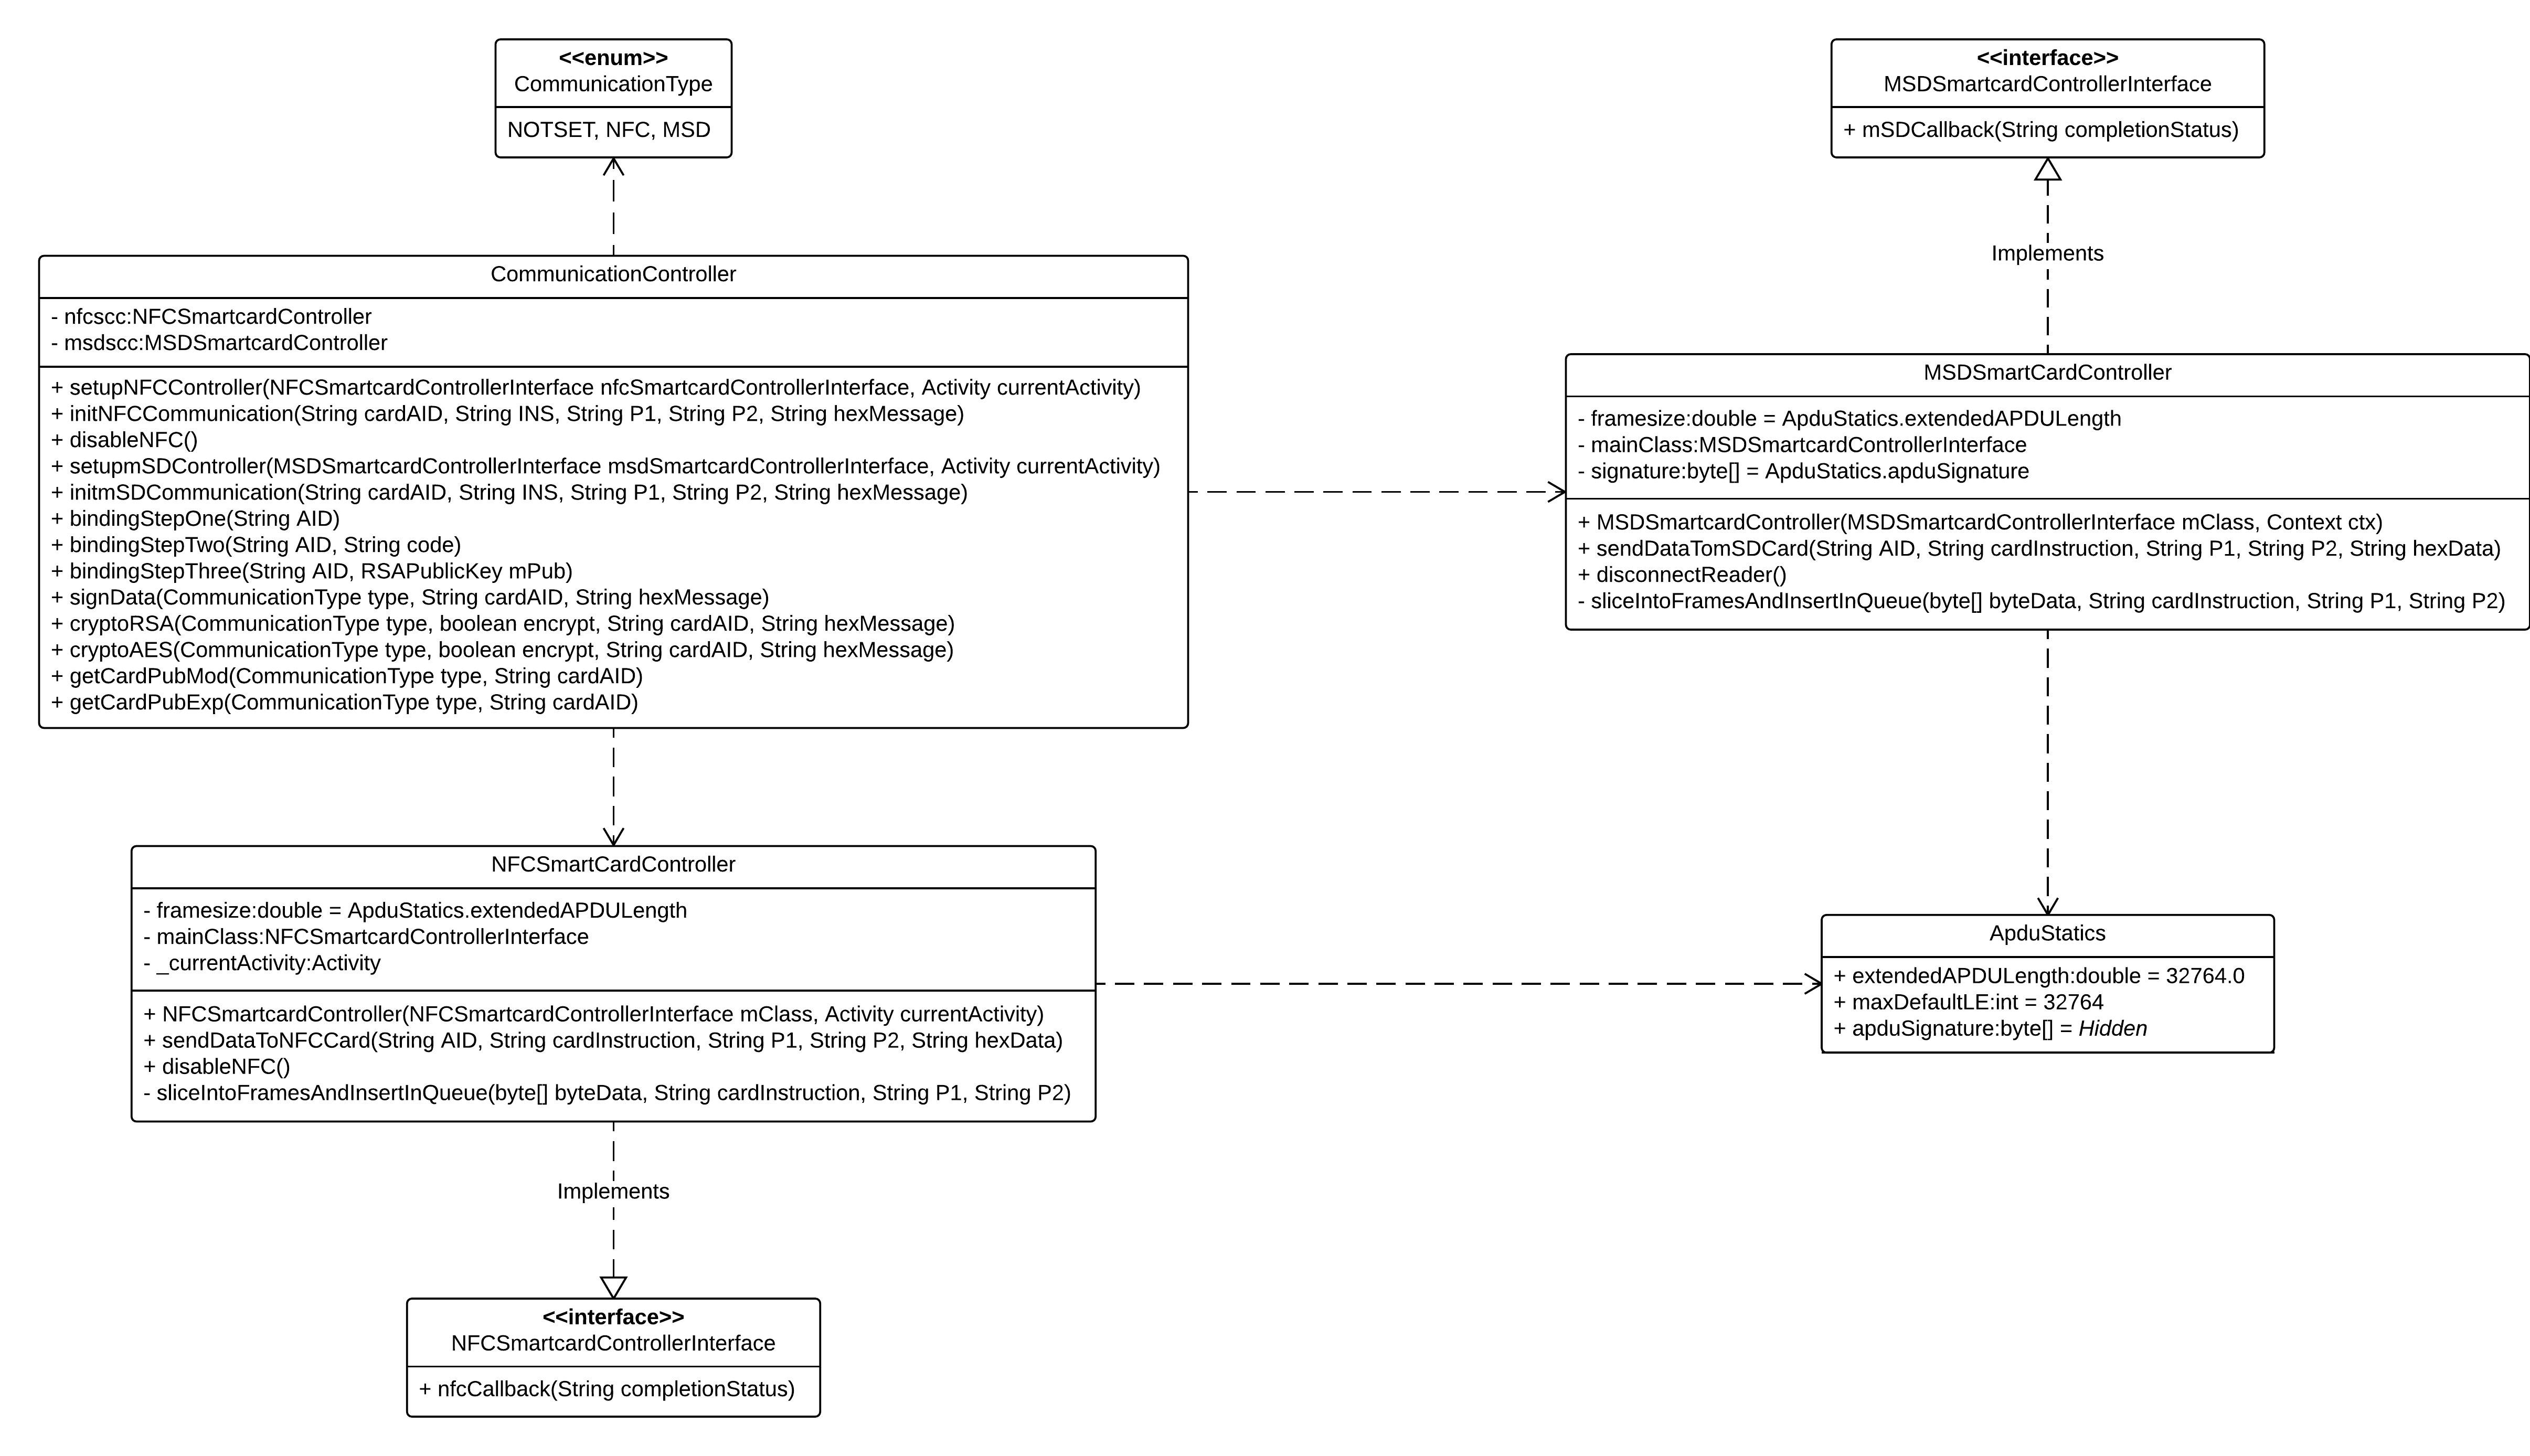
\includegraphics[width=1.25\textwidth, angle =90]{images/Class_Diagram.png}
\end{figure}
The package diagram, figure \ref{fig:package}, shows how  the packages in the library are structured.

\begin{figure}[h!]
  \caption{Library package diagram.}
  \label{fig:package}
  \centering
    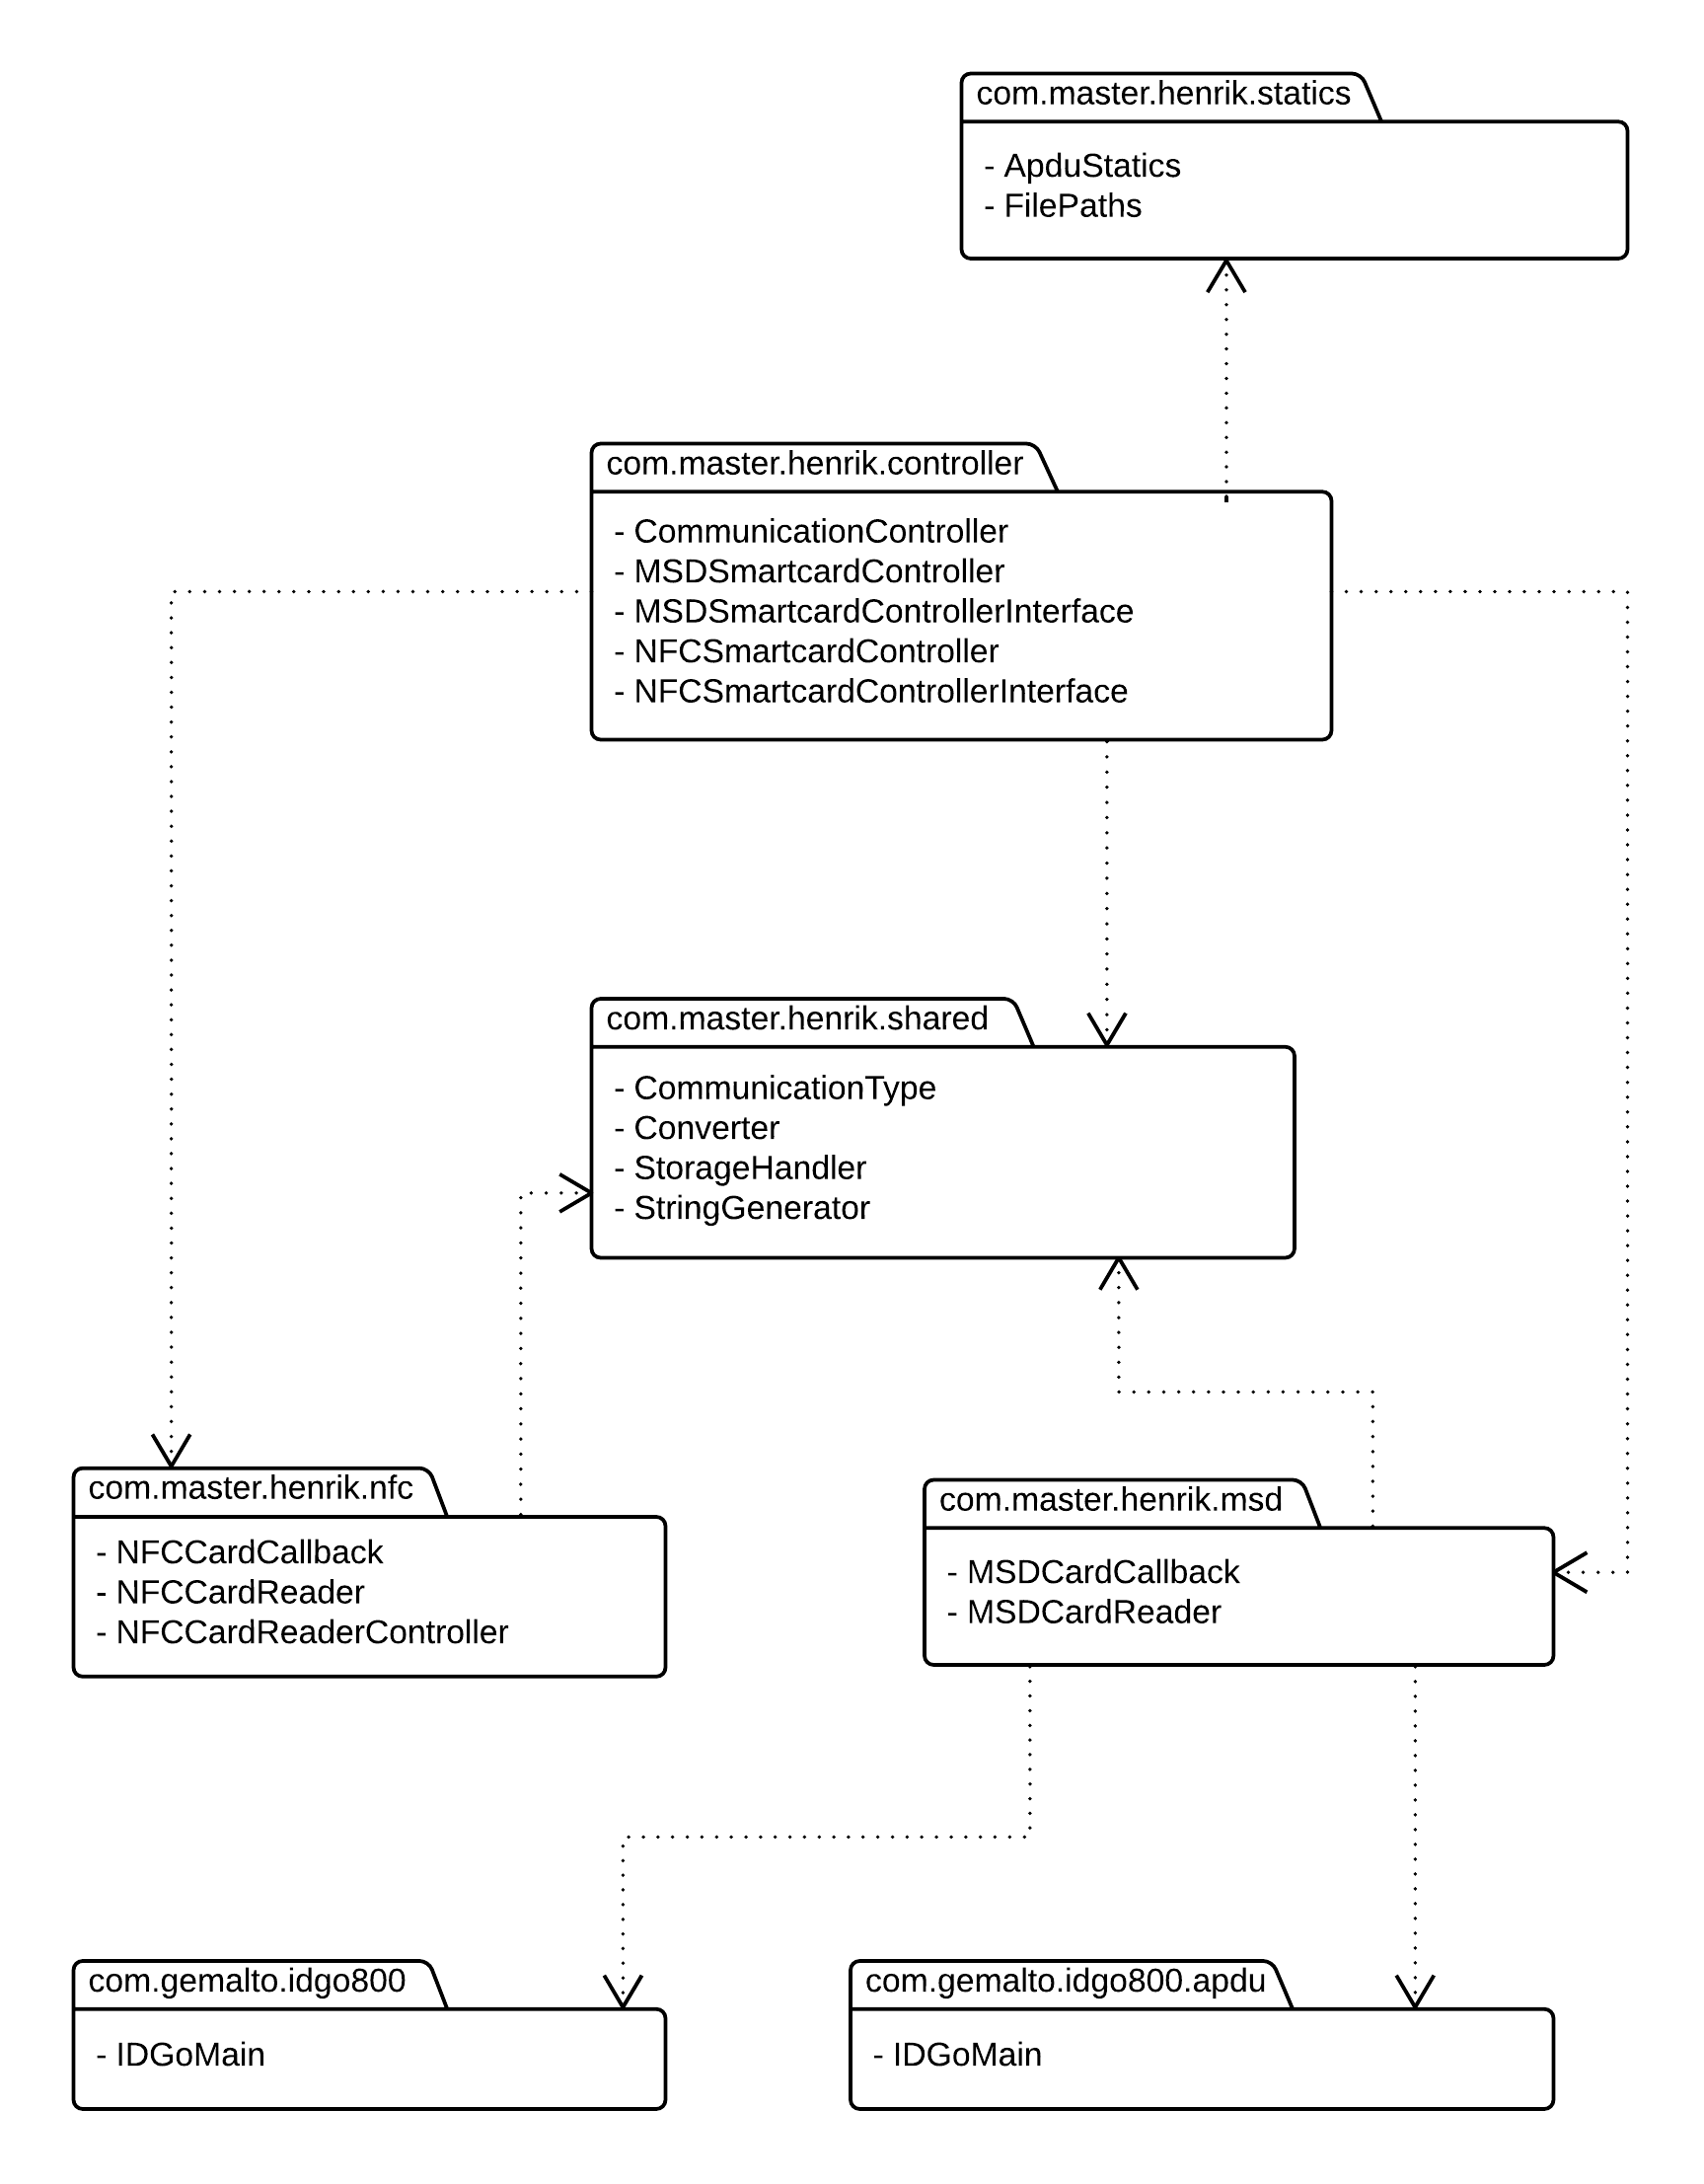
\includegraphics[width=0.95\textwidth]{images/package2.png}
\end{figure}
